\begin{figure}[htbp]
\centering
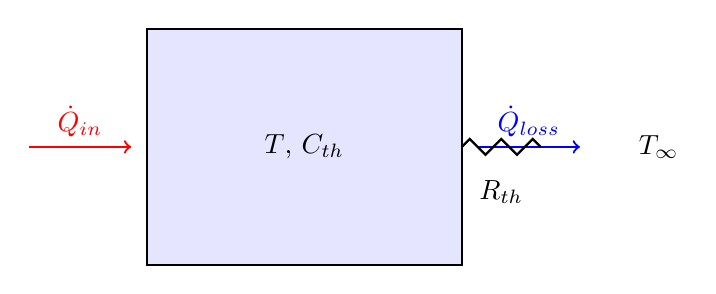
\begin{tikzpicture}
    % Room/body
    \draw[thick, fill=blue!10] (0,0) rectangle (4,3);
    \node at (2,1.5) {$T$, $C_{th}$};

    % Heater input
    \draw[->, thick, red] (-1.5,1.5) -- (-0.2,1.5) node[above, midway] {$\dot{Q}_{\text{in}}$};

    % Heat loss
    \draw[->, thick, blue] (4.2,1.5) -- (5.5,1.5) node[above, midway] {$\dot{Q}_{\text{loss}}$};

    % Ambient
    \node at (6.5,1.5) {$T_\infty$};

    % Thermal resistance
    \draw[thick, decorate, decoration={zigzag, segment length=4mm, amplitude=1mm}]
        (4,1.5) -- (5,1.5);
    \node[below] at (4.5,1.2) {$R_{th}$};
\end{tikzpicture}
\caption{Single-capacitance thermal system.}
\label{fig:single_thermal}
\end{figure}
